% Drawing 154/07-21 -- folder 154, batch 07, archive page 131 (PDF page 132).
% Transcription: en bas à droite, un cercle noir traversé d'un diamètre, les extrémités marquées $\alpha$ et $\alpha'$, une flèche de rotation
% Kind: circle with a diameter and a rotation arrow. Method 2 (schematic redraw from the facsimile). Status: ok.
% Notes: Thick black circle, a thin horizontal diameter with a heavy dot at each end; under each end a short stroke across the rim, lettered alpha on the left and alpha' on the right; a curved arrow outside the circle on the right, from the level of the diameter upwards. Overlaid on the 400 dpi colour crop on 2026-11-12: the diameter raised by 1 mm onto its ink, its two end dots and the two short strokes that carry alpha and alpha' added, the arrow put on its ink. Redrawn 2026-11-12 (issue 128): to check again. Overlay check 2026-11-13 (claude-opus-5-5, issue 128): the 300 dpi colour crop laid under the redraw compiled with tectonic. The whole figure lay about 1.5 mm up and to the left of its ink: circle, diameter (at y=-39, lower than the 2026-11-12 correction put it), end dots, the two short strokes, the letters and the arrow moved onto the page. Matches the facsimile.
% Coordinates: 1 unit = 1 mm = 1/100 of the crop width (bbox in page fractions: [0.785, 0.445, 0.925, 0.52]).
% Redrawn by Claude (claude-fable-5-2), issue #128, 2026-11-12; not checked by a human; not compiled (no TeX in the session).
% Corrected by Claude (claude-fable-5-2) 2026-11-12 (issue #128): overlaid on the 400 dpi colour facsimile and redrawn from it. Not compiled. Status: ok.
% Checked by Claude (claude-opus-5-5) 2026-11-13 (issue #128): overlaid on the 300 dpi colour facsimile and corrected; compiled with tectonic, no errors. Status: ok.
% Rights: reproduces part of the work -- behind RENDER_TRANSCRIPTS, never published by itself.
\documentclass[tikz,border=3pt]{standalone}
\usepackage{amsmath,amssymb}
\usetikzlibrary{patterns,arrows.meta}
\tikzset{pencil/.style={black!45}, struck/.style={black!35}, mpt/.style={circle,draw,inner sep=1.3pt}, pt/.style={circle,fill,inner sep=0.9pt}, opt/.style={circle,draw,fill=white,inner sep=1.1pt}}
\colorlet{Or}{orange!90!black}\colorlet{Ye}{yellow!80!orange}\colorlet{Lg}{green!60!black!70}\colorlet{Dg}{green!45!black}\colorlet{Br}{brown!80!black}\colorlet{Rd}{red!85!black}\colorlet{Bl}{blue!70!black}\colorlet{Gy}{black!40}
\begin{document}
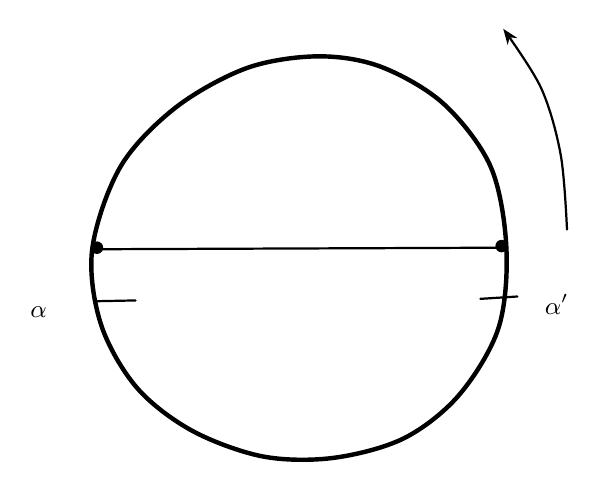
\begin{tikzpicture}[x=1mm,y=1mm,line cap=round,line join=round,font=\scriptsize]
\draw[line width=1.6pt] plot[smooth cycle, tension=0.55] coordinates {(48.6,-14.5) (39.6,-16) (30.6,-21) (23.6,-28.5) (20,-39) (21.1,-48.5) (25.6,-56.5) (32.6,-62) (41.6,-65.3) (50.6,-65.5) (59.6,-63) (66.6,-57.5) (71.6,-49) (72.6,-38.8) (70.6,-28.5) (64.6,-20.5) (56.6,-15.8)};
\draw[thick] (20,-39) -- (72.6,-38.8);
\node[pt,inner sep=1.6pt] at (20.6,-38.8) {};
\node[pt,inner sep=1.6pt] at (72,-38.6) {};
\draw[thick] (20.5,-45.6) -- (25.5,-45.5);
\draw[thick] (69.3,-45.3) -- (74,-45);
\node[inner sep=1pt] at (13.2,-47) {\small $\alpha$};
\node[inner sep=1pt] at (79,-46) {\small $\alpha'$};
\draw[thick,-{Stealth[length=2mm]}] plot[smooth, tension=0.55] coordinates {(80.3,-36.5) (79.5,-27) (77,-18.5) (72.2,-11)};
\end{tikzpicture}
\end{document}
